%DataMiningAndPredictiveAnalytics
%TODO: talk about why data mining and clustering is now so important, since so much data - also mentioned in data mining concepts.. book on page 363
%THERE ARE CASE STUDIES AT THE END OF THIS BOOK
\textcite{DataMiningAndPredictiveAnalytics}[4] declare, that data mining is used to recognise patterns and trends in large amounts of data. \textcite{han2011data}[16-18] explain, that the term "data mining" is a misnomer. A more suitable phrase would be "knowledge mining from data". The word "mining" represents valuable nuggets found within large amounts of raw material. Other names used to describe the same process include: knowledge discovery from data (KDD), knowledge extraction, data/pattern analysis, data archaeology, and data dredging.
According to the authors, the discovery of data is an iterative process represented in the following steps: Data cleaning, data integration (combine multiple data sources), data selection (relevant data is extracted), data transformation (into applicable forms for data mining), data mining (discover patterns), pattern evaluation (determine if patterns have a meaning), and knowledge presentation. The following data forms, are typically used for mining: database data, data warehouse data, and transactional data. Other forms include data streams, ordered/sequence data, graph or networked data, spatial data, text data, multimedia data, and the World Wide Web. Data mining requires continuous human supervision for quality monitoring and evaluation, as stated by \textcite{DataMiningAndPredictiveAnalytics}[9-13, 15-16]. Software alone will serve wrong results. Data mining is used for description of patterns and trends, estimation of numerical values, prediction of future results, classification of categorical variables, clustering of similar objects and association of attributes. 

\textcite{DataMiningAndPredictiveAnalytics}[160] describe the two types of data mining methods: \textit{supervised} and \textit{unsupervised}. \textcite{han2011data}[363] interpret supervised learning as \textit{learning by examples}, whereas unsupervised learning is \textit{learning by observation}. \textcite{DataMiningAndPredictiveAnalytics}[160-163] continue, the majority of methods are supervised. In supervised methods, there is a predefined target variable. The method receives several examples, where the target variable value is defined, thus learning which values of the target variable correspond to which values of the predictor variable. The goal of the unsupervised approach is to find patterns and structure in the inserted variables. Therefore, no target variable is established. Clustering is the most prevalent unsupervised method. As reported by \textcite{han2011data}[32], through using unsupervised machine learning, it is possible to detect classes within data.

Problems that can occur in data mining methods are data dredging, underfitting and overfitting. As stated in \textcite{DataMiningAndPredictiveAnalytics}[160-163], data dredging arises when false results develop in data mining due to random variations of data. Cross-validation is used to prevent data dredging, by guaranteeing that the results can be generalised to an independent data set. 

In their paper on attempting to balance underfitting and overfitting, \textcite{van2010process}[87-89] clarify when these can occur. When fitting a model to a log, underfitting or overfitting the model are main problems. Underfitting the model means not fitting the model well enough to the log, therefore allowing too much behaviour which is not present in the log ("anything is possible"). Overfitting has the opposite effect. The model is fitted too well to the log, thus reducing it to another depiction of the log. It therefore only permits the same paths present in the log. These problems can take effect, for example, in a hospital process. Each patient's path of events is most probably unique, two patients are unlikely to have the same process. Hence, the event log is always growing, therefore generalisation is required to avoid overfitting. Likewise, underfitting (allowing all possibilities) should also be averted. 
\textcite{DataMiningAndPredictiveAnalytics}[164-165] mention, that another way to describe the overfitting/underfitting problem is through the bias-variance trade-off. In figure \ref{figure:biasTradeOff} there are three scatter plots with data points in two different colours, which need to be separated by a line. The first scatter plot depicts a low-complexity separator (e.g. a straight line), which may have some classification errors (\textit{high bias}), however it needn't change much to accommodate new data points. Therefore, it has \textit{low variance}. The second scatter plot illustrates a high-complexity separator (e.g. curvy line that can separate more of the points correctly), which reduces the amount of errors (\textit{low bias}), but has to change a lot when new data points are added. Thus, it has \textit{high variance}. The higher the complexity of the model gets, the bias is reduced, the variance however increases. The third scatter plot shows both a low-complexity separator and a high one, with additional data. While the low-complexity separator can can still classify with little change, the high-complexity one needs to be altered more. The ideal model has neither high bias or variance.

\begin{figure*}[h]
  \centering
  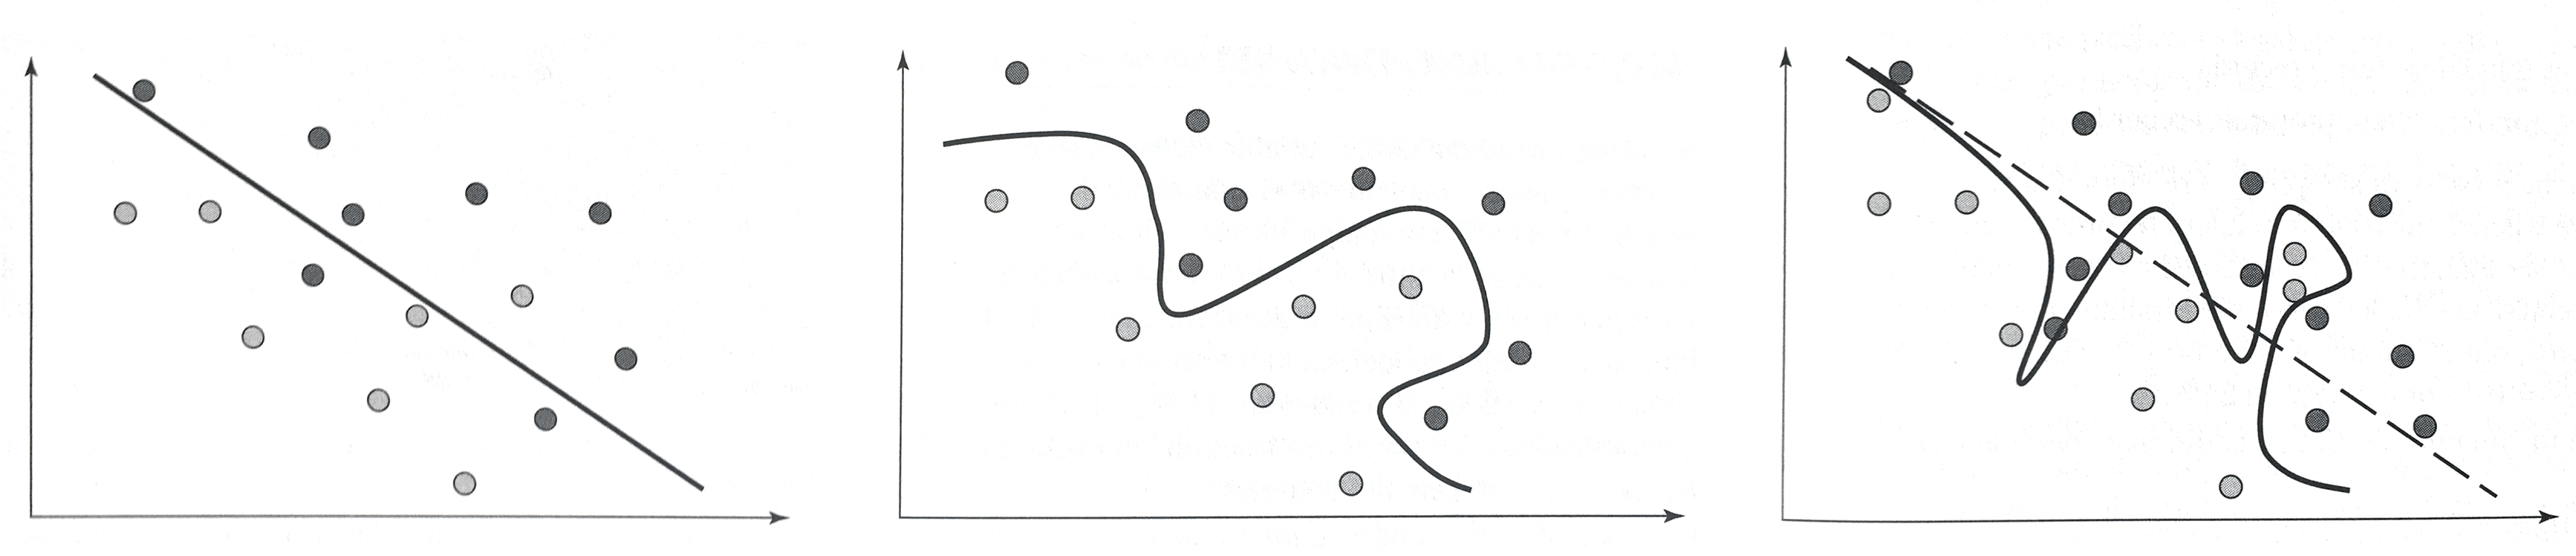
\includegraphics[width=1\textwidth]{./images/biasTradeOff.png}
  \caption{These three scatter plots from \textcite{DataMiningAndPredictiveAnalytics}[164-165] depict the bias-variance trade-off. The first plot portrays a low-complexity resulting in a high error rate. The second plot achieves a low error rate by using a high-complexity separator. The third graph compares the two separators.
  }
  \label{figure:biasTradeOff}
  
\end{figure*}


%BOOK Data mining concepts and techniques
%page 12 and 13 explains how much data exists, goes through google, basically why we need data mining


%page 18 - another sentence explaining what data mining is, but similar to one from other book
%page 18


%page 28, 29 - outlier analysis



%page 32 - there is an example for unsupervised m. l. on this page, but not really sure if need it


%page 416




%TODO: EXPLAIN HOW TO NORMALIZE - PAGE 105 OF DATA MINING CONCEPTS.. BOOK -> also explained in data mining and predictive analysis - page 94

%TODO:  data mining concepts and techniques: outlier detection p445, and "Data mining trends and research frontiers" p481